\documentclass{scrreprt}

\usepackage[croatian]{babel}
\usepackage[utf8]{inputenc}
\usepackage[T1]{fontenc}
\usepackage{hyperref}
\usepackage{graphicx}
\usepackage{tikz}
\usepackage{pgfplots}
\usepackage{float}
\usepackage[nottoc,numbib]{tocbibind}
\usepackage{color}
\usepackage{multicol}
\usepackage[export]{adjustbox}
\usepackage{url}
\usepackage[stable]{footmisc}

\setlength{\parskip}{\bigskipamount}
\setlength{\parindent}{0pt}

\graphicspath{ {./images/} }

\begin{document}

\titlehead{\center{Sveučilište u Zagrebu\\Filozofski fakultet\\Odsijek za
informacijske i komunikacijske znanosti\\Akademska godina 2013/14.}}
\title{Upotreba web aplikacije za kvizove u nastavi osnovnih i srednjih škola}
\author{Studenti: Janko i Matija Marohnić\\Mentor: doc.dr.sc. Kristina Kocijan}
\date{Zagreb, 2014.}

\maketitle

\pagebreak

Ovaj rad izrađen je na Odsijeku za informacijske i komunikacijske znanosti na
Filozofskom fakultetu u Zagrebu pod vodstvom prof.dr.sc. Kristine Kocijan i
predan je na natječaj za dodjelu Rektorove nagrade u akademskoj godini
2013/2014.

\pagebreak

\tableofcontents

\chapter{Uvod}

Zbog sveprisutnosti tehnologije i interneta mnogi učenici imaju sve više
poteškoća s učenjem, odnosno sve manje koncentracije i motivacije, i često ne
vide smisao u učenju jer većinu informacija vrlo brzo mogu pronaći na internetu.
To je zato što se sustav školovanja već dugo nije promijenio, a generacije
jesu.\cite{perisic13} Zato učenici često uzimaju instrukcije kako bi imali bolje
ocjene, jer im je potreban alternativni način podučavanja kojeg ne nalaze u
školama.\cite{kustura09}

Postoje razni kreativni načini da se upotrijebi informacijska tehnologija u
nastavi:

\begin{itemize}
  \item prezentacije (npr. koristeći program kao što je \emph{Microsoft
    PowerPoint})
  \item ilustracije
  \item digitalne simulacije (npr. u fizici)
  \item video zapisi (npr. preko servisa kao što je \emph{YouTube} ili
    \emph{Vimeo})
  \item itd.
\end{itemize}

Međutim, to je obično prilično jednostrano, u smislu da samo profesori koriste
tehnologiju dok ih učenici gledaju. Ljudi bolje uče i više se interesiraju za
gradivo kroz interakciju. Smatramo da se trebaju razvijati puno interaktivnije i
zabavnije metode podučavanja.

Profesori koji su spremni koristiti interaktivne alate za podučavanje nemaju velik
izbor jer je većina dobrih alata na engleskome jeziku, što predstavlja problem
mlađoj djeci koja još ne znaju dobro engleski, ili starijim profesorima koji ga
nikada nisu trebali dobro ni znati. Potreban je jednostavan alat koji je
namijenjen hrvatskoj populaciji.

Jedna od najjednostavnijih načina ispitivanja znanja je riješvanje kvizova,
stoga smo pretraživali hrvatske i strane aplikacije koje se bave tom temom, pa
ćemo ih navesti i opisati nekoliko.

\begin{description}

  \item[Kvizovi.net]\footnote{\url{http://kvizovi.net}} je srpska aplikacija za
    kvizove iz mnogih područja, kao što su glazba, zemljopis, sport, povijest,
    filmovi i serije. Osim kvizova ima i igara i viceva, ali kompletan sadržaj
    ove aplikacije je vrlo siromašan zbog toga što ju mogu izmjenjivati jedino
    autori aplikacije, nema baze korisnika koji mogu stvarati i riješavati
    kvizove, pa prema tome skupljati bodove i sl.

  \item[Kvizoteka]\footnote{\url{http://www.kvizoteka.net}} je, kao i
    \emph{Kvizovi.net}, kolekcija besplatnih kvizova iz svih područja kao što su
    filmovi, povijest, opće znanje, sport, glazba itd. Osim kvizova, nudi i
    popularne igrice kao što su Pacman, Tetris, Super Mario itd. Za razliku od
    \emph{Kvizovi.net}, \emph{Kvizoteka} ima bazu korisnika i neke statističke
    informacije o kvizovima.

  \item[Učionica]\footnote{\url{https://itunes.apple.com/hr/app/ucionica/id566902215?mt=8}}
    je iOS\footnote{Mobilni operacijski sustav kojeg razvija Apple.} aplikacija
    namijenjena djeci predškolske dobi, pomaže im svladati osnovne pojmove kao
    što su abeceda, životinje, brojevi, oblici, boje i vrijeme. Iako se
    riješenje koje mi tražimo odnosi na djecu osnovnoškolske i srednjoškolske
    dobi, ova aplikacija je dobar primjer hrvatske aplikacije učenja kroz igru.
    Nedostatak joj je to što je dostupna samo za iOS, nije ju još moguće
    koristiti na ostalim mobilnim operacijskim sustavima, niti na desktop ili
    laptop računalima.

  \item[QuizUp]\footnote{\url{https://itunes.apple.com/hr/app/quizup/id718421443?mt=8}}
    je vrlo kvalitetna i popularna aplikacija za kvizove na engleskom jeziku. Od
    navedenih, ova aplikacija je najviše opsežna i ažurna i ima najviše značajki
    (eng. \emph{feature}). Osim riješavanja kvizova, korisnici \emph{QuizUp}-a
    ih mogu i stvarati ako žele. Za razliku od ostalih navedenih aplikacija,
    \emph{QuizUp} ima puno izraženiji socijalni aspekt i upotrebu
    gejmifikacije\footnote{Korištenje elemenata iz igara u drugim kontekstima.},
    koja potiče riješavanje kvizova, tako što korisnici dobivaju bodove i prema
    njima im se dodjeljuju određeni statusi. Nedostaci ove aplikacija su
    engleski jezik i što je dostupna samo na mobilnim uređajima, nije ju moguće
    igrati na desktop i laptop računalima.

\end{description}

S obzirom da nismo našli nijedno prihvatljivo riješenje za hrvatsku aplikaciju
za kvizove, počeli smo razvijati svoju i nazvali smo ju
\emph{Kvizovi}\footnote{\url{http://kvizovi.org}}. To je aplikacija za
riješavanje kvizova koja je prilagođena osnovnim i srednjim školama u Hrvatskoj.
Prepoznaje 2 osnovna tipa korisnika -- \textbf{učenike} i \textbf{profesore}. U
ovom smo istraživanju testirali \emph{Kvizove} na nekoliko osnovnih i srednjih
škola.

\chapter{Hipoteza}

Cilj ovog istraživanja bio je saznati:

\begin{enumerate}
  \item pomaže li takav način učenja učenicima da bolje savladaju gradivo
  \item čini li aplikacija profesorima podučavanje zanimljivijim
\end{enumerate}

Pretpostavljamo je da će se više zainteresirati za gradivo te ga bolje usvojiti
oni učenici koji su ga učili riješavajući kvizove pomoću aplikacije od onih koji
nisu. Učenici riješavanje kvizova mogu gledati kao neku vrstu igre, što može
pozitivno utjecati na usvajanje znanja. Interes za gradivo može potaknuti
mogućnost igranja u paru, odnosno natjecanja s drugim učenicima.

Druga pretpostavka je da će profesorima ispitivanje učenika pomoću aplikacije za
kvizove biti jednostavnije i informativnije nego ispitivanje na tradicionalne
načine kao što su sastavljanje testova i usmeno ispitivanje. Može biti
jednostavnije zato što kviz trebaju sastaviti jednom i mogu koristiti alat koji
je specijaliziran za kvizove, ne moraju ih tiskati i ne moraju ih ručno
ispravljati kasnije, nego se to događa automatski prema točnim odgovorima koje
su profesori unijeli. A može biti informativnije zato što profesori dobivaju
puno podataka o tome kako njihovi učenici riješavaju kvizove, koliko im je
trebalo za svako pitanje, kada su točno bili gotovi, s kime su igrali itd.

Valja uzeti u obzir da prema VAK principu postoje 3 različita tipa ljudi --
vizualni, auditivni i kinestetički.\cite{clark11} Smatramo da će naša aplikacija
najviše pomoći onima koji najbolje uče preko vizualnih i kinestetičkih
podražaja.

\chapter{Sredstva i metode}

Istraživanje smo proveli tako što smo izradili aplikaciju za kvizove i dali
određenom uzorku osnovnih i srednjih škola na testiranje. Podatke o kvizovima
skupljali smo 2 godine. U svakom razredu su učenici bili podijeljeni na skupinu
koja ne riješava kvizove i na onu koja riješava, na taj način smo mogli
provjeravati učinkovitost aplikacije kada bi učenici imali test znanja. Imamo
puno podataka na raspolaganju, ali smo za svaki slučaj proveli još i ankete kako
bismo dobili podatke koje pasivno ne bismo mogli dobiti.

Imamo blog na kojemu obaviještavamo korisnike o ažuriranju aplikacije. S obzirom
da je dio ciljane publike starija populacija koja nije nužno iskusna s
aplikacijama, dodali smo i vodič kroz aplikaciju koji je dostupan u bilo kojem
trenutku, kako bi se korisnici lakše snašli. Također, u slučaju da ima nekih
problema, korisnici nas uvijek mogu kontaktirati putem e-mail adresa koje se
nalaze u kontakt sekciji koju smo stavili u glavnu navigaciju. Korisnici također
mogu naknadno izmjenjivati svoje podatke u korisničkom računu.

Korisnik započinje korištenje aplikacije tako da odabere svoju ulogu u školi,
stoga ovisno o ulozi aplikacija pruža drugačiju funkcionalnost.

\begin{figure}[H]
  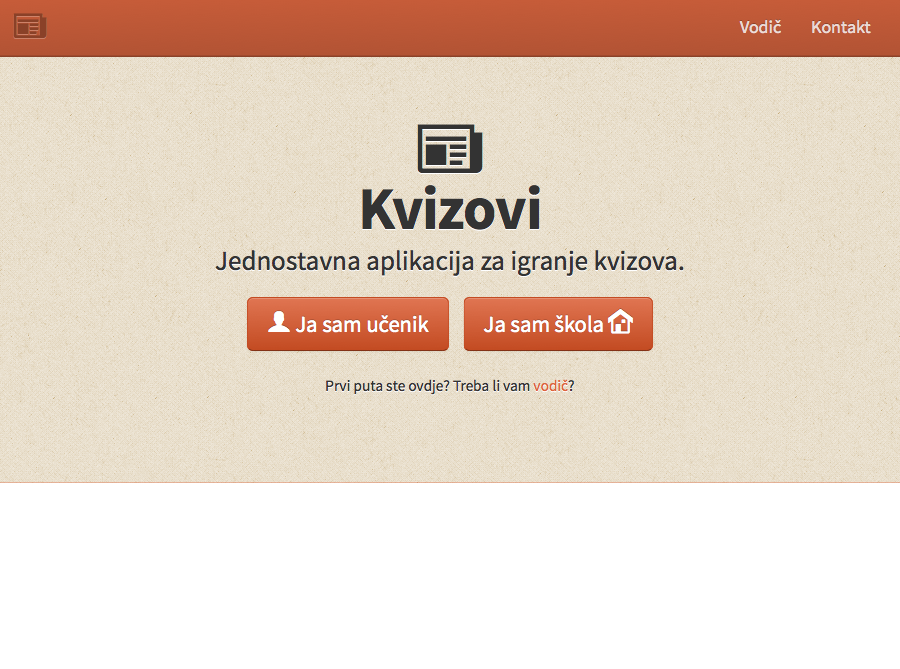
\includegraphics[width=\textwidth, clip=true, trim=0 7cm 0 0, fbox]{home}
  \caption{Početna stranica}
\end{figure}

\section{Škola}

\emph{Škola} je uloga koja predstavlja profesora i ona je administrator kvizova.

% S obzirom na uzrast...

Nakon odabira te uloge korisnik se može prijaviti ili registrirati ako još nema
korisnički račun. Registracija se sastoji od ispunjavanja jednostavnog formulara
pomoću kojega skupljamo informacije o korisnicima koje možemo iskoristiti kako
bismo poboljšali njihovo iskustvo i kako bismo mogli raditi istraživanja. Polje
u formularu za registraciju na koje ćemo se osvrnuti je \emph{Tajni ključ}, koji
je potreban za registraciju učenicima te škole.

Nakon prijave profesore dočeka lista kvizova koje su napravili,

\begin{figure}[H]
  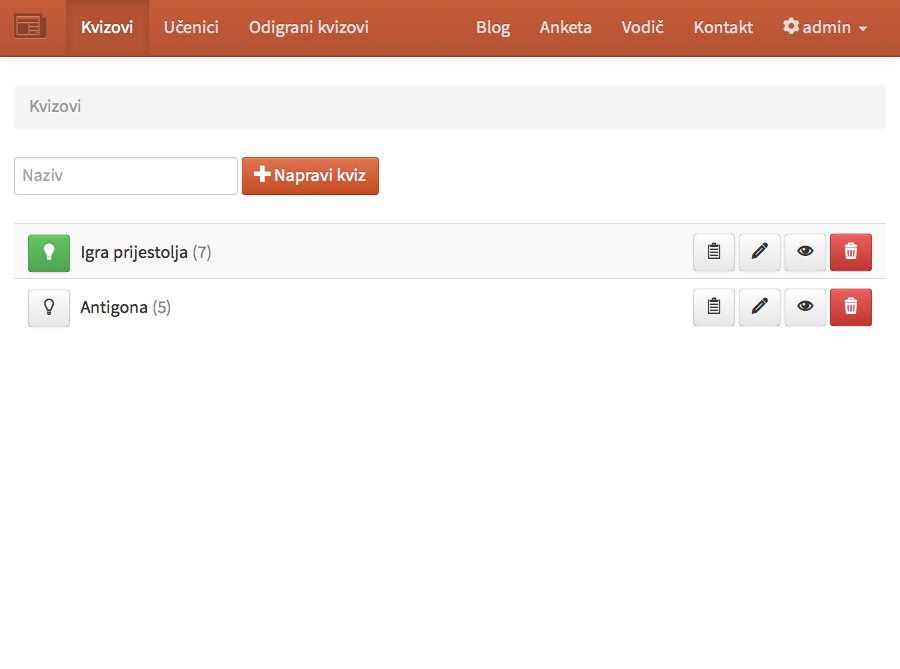
\includegraphics[width=\textwidth, clip=true, trim=0 10cm 0 0, fbox]{school/quizzes}
  \caption{Škole -- popis kvizova}
\end{figure}

gdje mogu izmjenjivati postojeće kvizove i sastavljati nove. Nakon što je
profesor zadovoljan s kvizom, može ga učiniti aktivnim, odnosno vidljivim
učenicima. Izmjenjivanje kvizova podijeljeno je na izmjenu metapodataka kviza i
na izmjenu pitanja kviza.

\begin{figure}[H]
  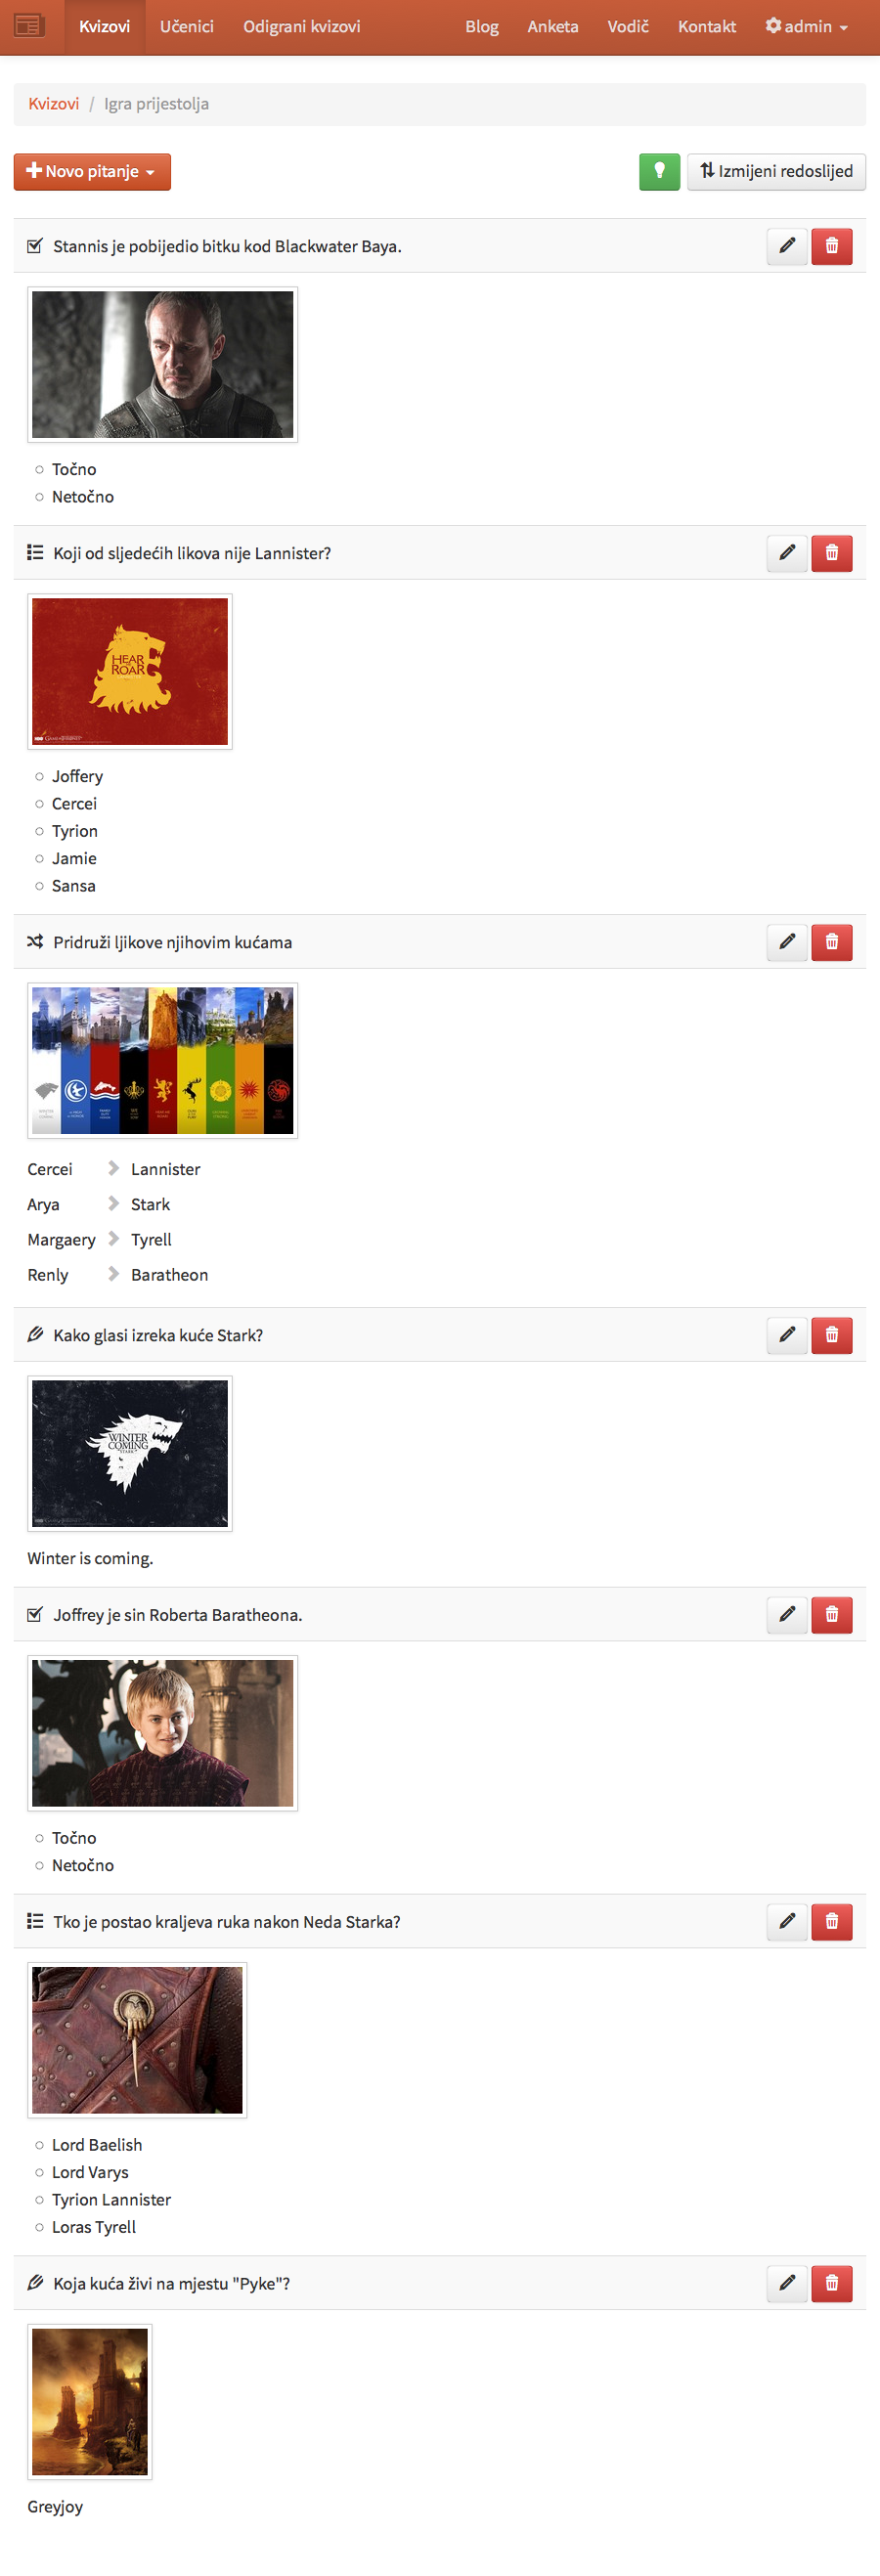
\includegraphics[width=\textwidth, clip=true, trim=0 53cm 0 0, fbox]{school/quiz}
  \caption{Škole -- popis pitanja u kvizu}
\end{figure}

Postoji 4 vrsta pitanja:

\begin{itemize}
  \item Točno/netočno
  \item Ponuđeni odgovori
  \item Asocijacija
  \item Upiši točan odgovor
\end{itemize}

Uz svako se pitanje može pridružiti pomoć, koja će se prikazati učenicima dok
riješavaju pitanje.

Škole mogu pregledavati informacije o odigrane kvizove, kada su igrani, tko ih
je igrao, koji su bili rezultati itd.

\begin{figure}[H]
  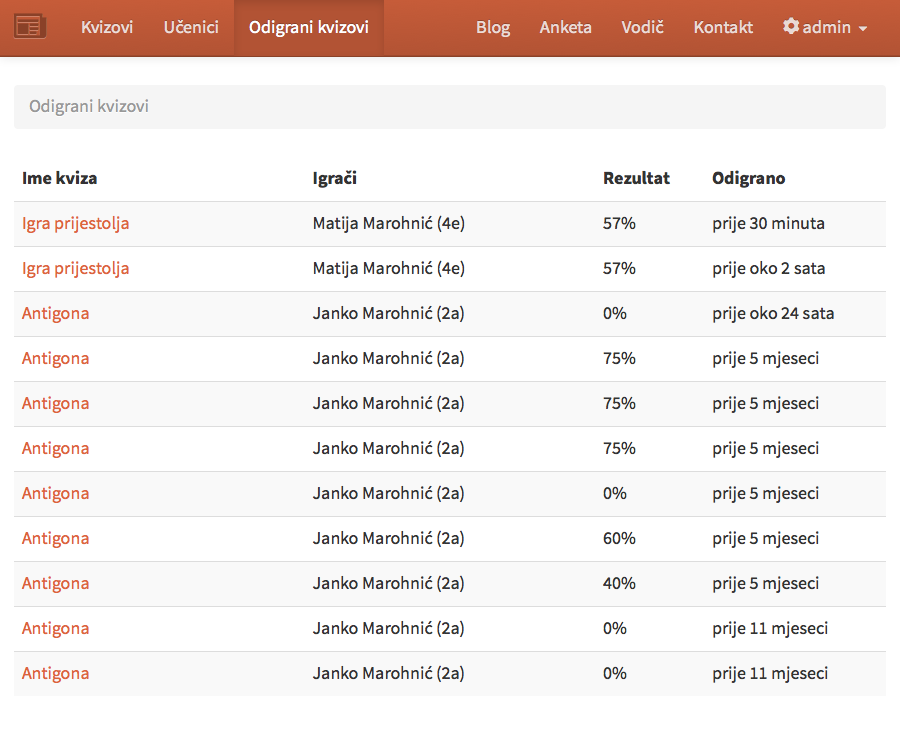
\includegraphics[width=\textwidth, clip=true, trim=0 10cm 0 0, fbox]{school/played_quizzes}
  \caption{Škole -- popis odigranih kvizova}
\end{figure}

\begin{figure}[H]
  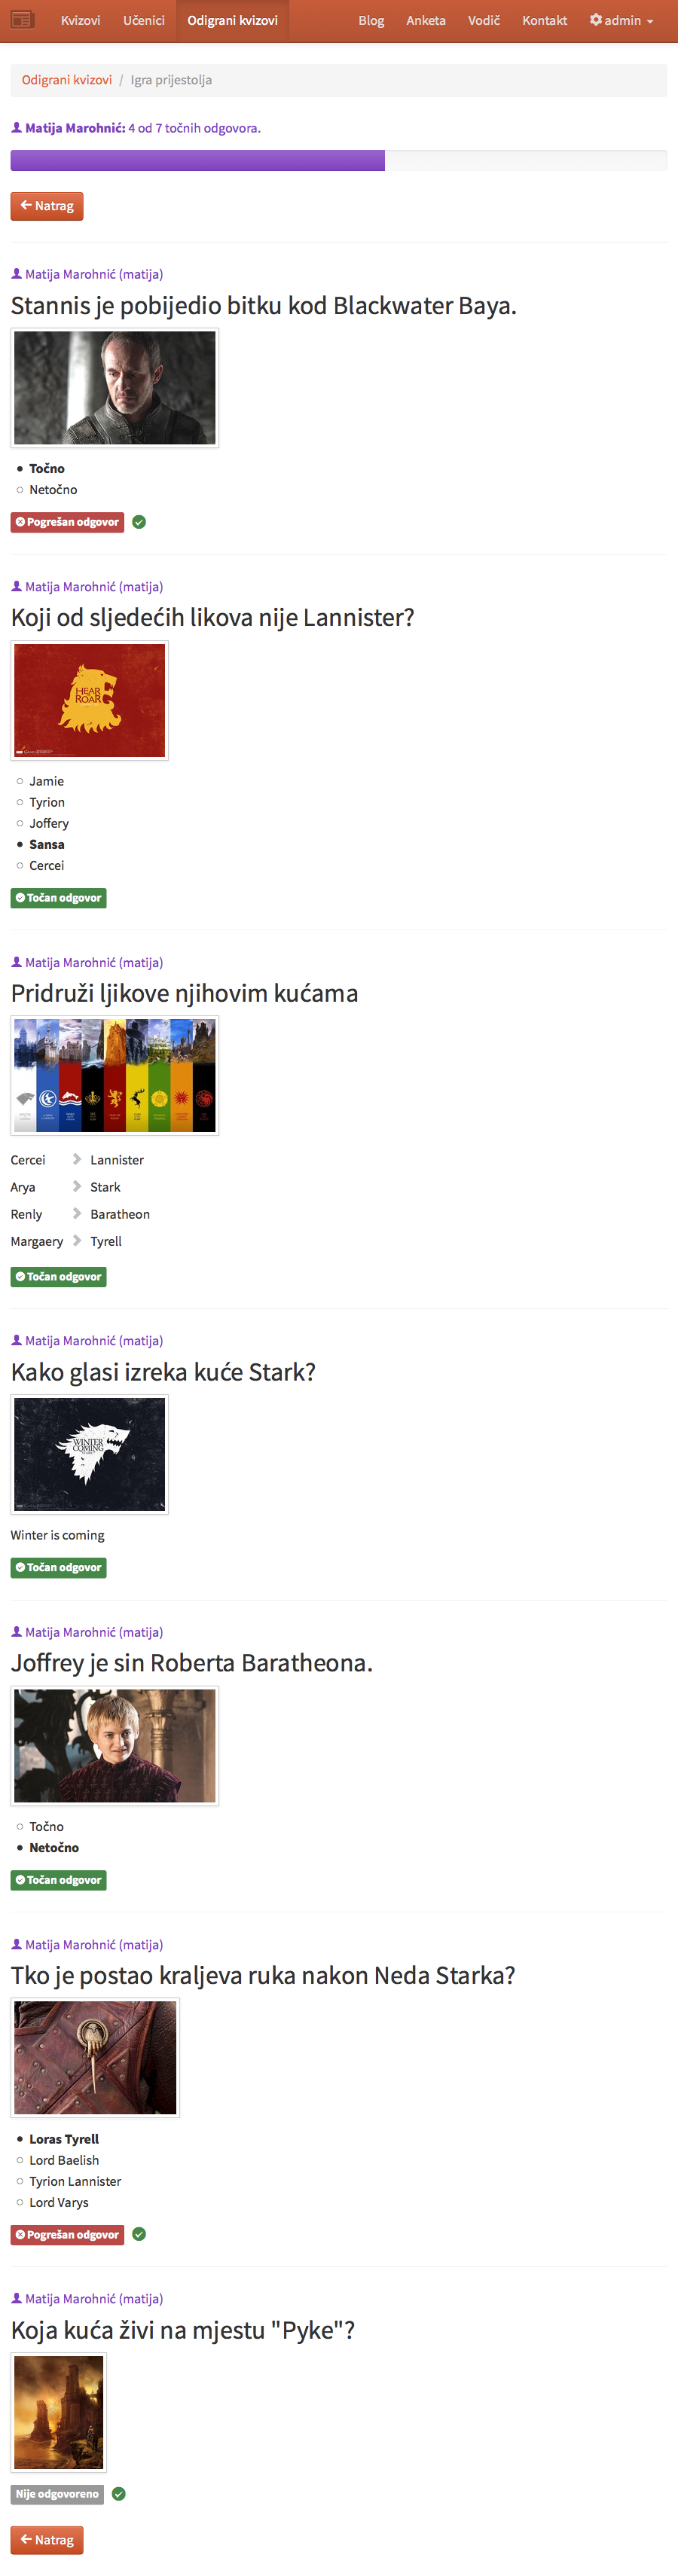
\includegraphics[width=\textwidth, clip=true, trim=0 80cm 0 0, fbox]{school/played_quiz}
  \caption{Odigrani kviz}
\end{figure}

Mogu se pregledavati i učenici, koliko su kvizova odigrali, koji su to kvizovi i
sl.

\begin{figure}[H]
  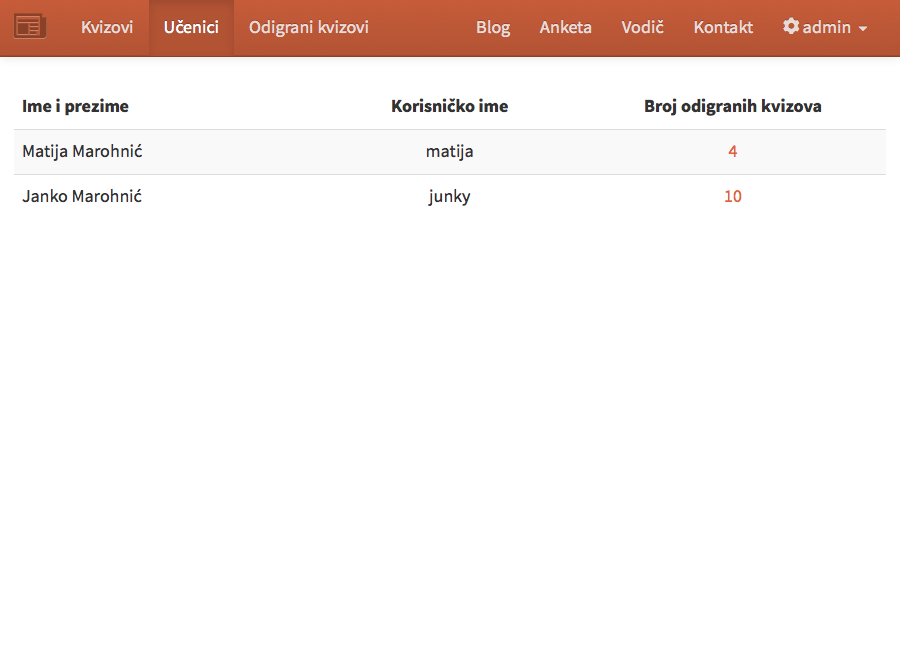
\includegraphics[width=\textwidth, clip=true, trim=0 15cm 0 0, fbox]{school/students}
  \caption{Škole -- popis učenika}
\end{figure}

\section{Učenik}

% S obzirom na uzrast...

\emph{Učenik} je uloga koja riješava kvizove koje je napravila njihova škola.
Kao i kod škole, učenik se može prijaviti ili registrirati, ako već nema
korisnički račun. Pri registraciji učenik treba napisati tajni ključ koji mu je
njegova škola dala, u protivnom se ne može registrirati. Na taj način
spriječavamo da se bilo tko registrira kao učenik.

Nakon prijave ili registracije, korisnika dočeka lista kvizova koji su dostupni
za riješavanje. Kviz je moguće igrati sam ili u paru, u drugom slučaju se drugi
igrač također treba prijaviti.

\begin{figure}[H]
  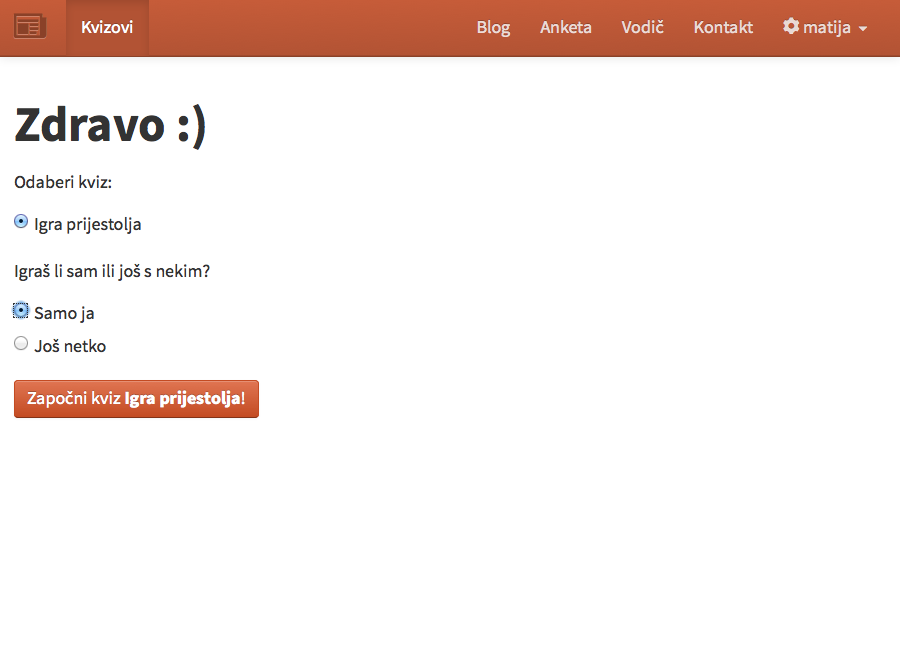
\includegraphics[width=\textwidth, clip=true, trim=0 8.5cm 0 0, fbox]{student/quizzes}
  \caption{Učenici -- popis kvizova}
\end{figure}

Nakon što učenik započne kviz, prikazuje mu se jedno po jedno pitanje na koja
treba odgovoriti. Kako bi igra bila što poštenija, pitanja su obično vremenski
ograničena, tako da se učenik ne stigne previše konzultirati s vanjskim
izvorima.

\begin{figure}[H]
  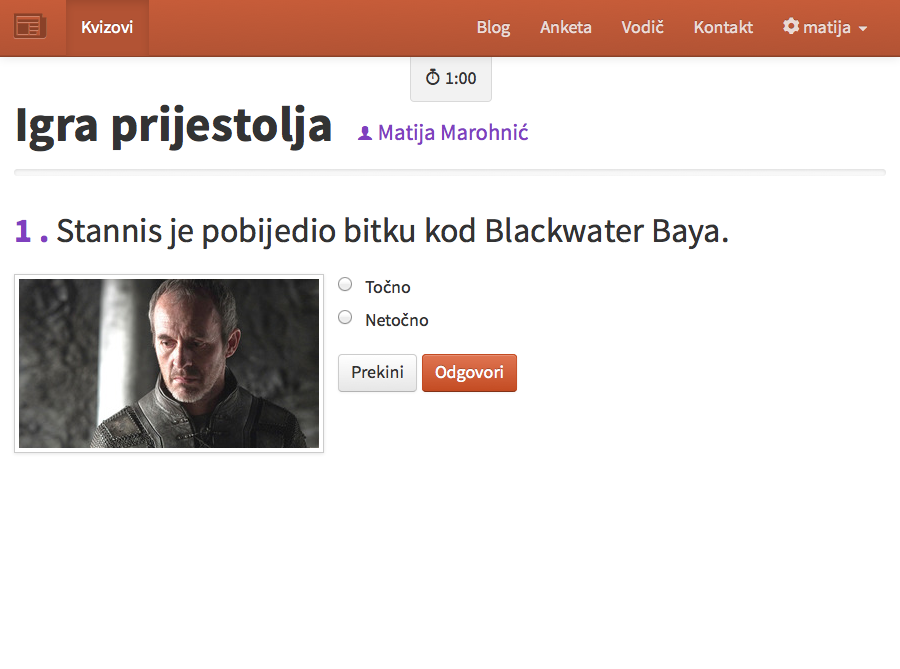
\includegraphics[width=\textwidth, clip=true, trim=0 7cm 0 0, fbox]{student/boolean_question}
  \caption{Učenici -- točno/netočno}
\end{figure}

\begin{figure}[H]
  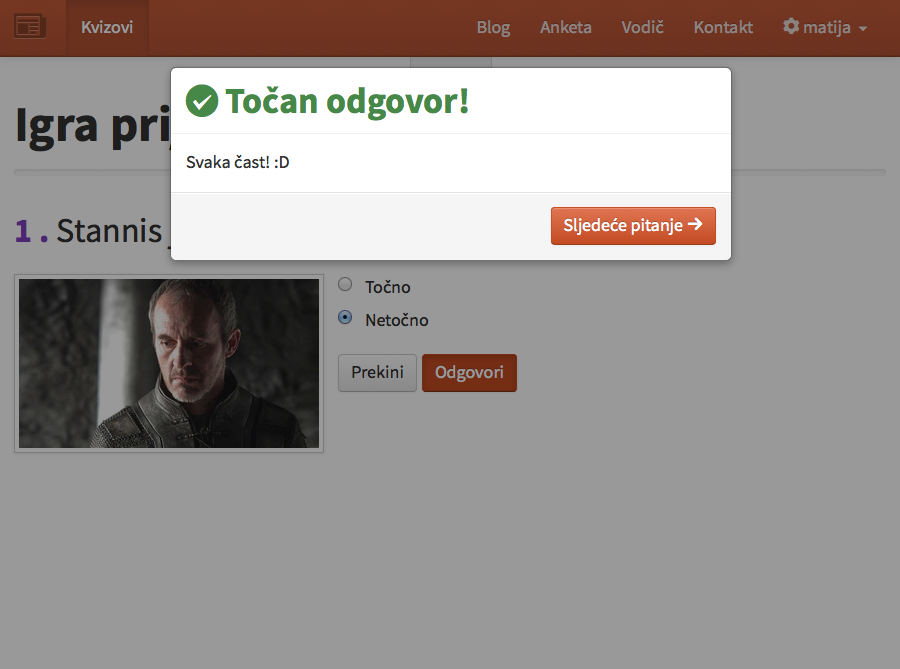
\includegraphics[width=\textwidth, clip=true, trim=0 7cm 0 0, fbox]{student/boolean_question_correct}
  \caption{Učenici -- točno/netočno s povratnom informacijom}
\end{figure}

Nakon što učenik odgovori na sva pitanja, ispisuju se rezultati i učenik dobiva
određenu ``titulu'' s obzirom na njegov rezultat. Titule su osmišljene tako da
se učenika uvijek pohvaljuje, čak i ako je imao loš rezultat, tako da se učenik
dobro osjeća i da ga se potiče da igra i dalje.


\chapter{Rezultati}

Ovo istraživanje pokazalo je da je većina profesora primjetila napredak u
poznavanju gradiva kod svojih učenika, kao i veću zainteresiranost za gradivo.

\begin{figure}[H]
  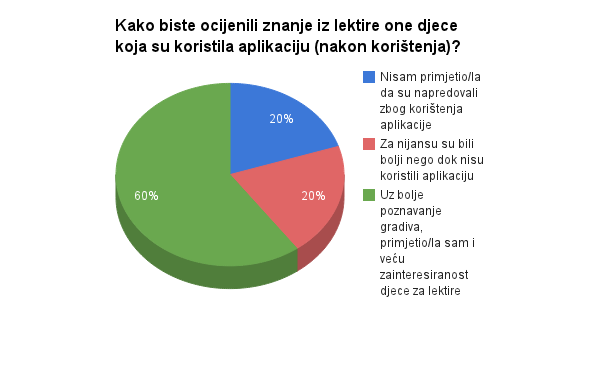
\includegraphics[width=\textwidth, clip=true, trim=0 2.5cm 0 0]{advance}
  \caption{Napredak učenika}
\end{figure}

\begin{figure}[H]
  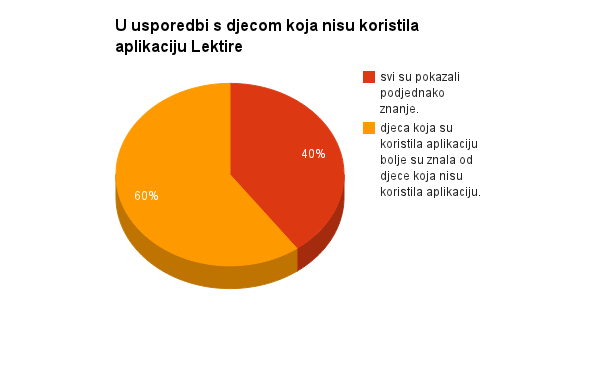
\includegraphics[width=\textwidth, clip=true, trim=0 2.5cm 0 0]{comparison}
  \caption{Usporedba učenika koji su koristili aplikaciju s onima koji nisu}
\end{figure}

\chapter{Rasprava}

% Namjeravamo otvoriti aplikaciju za sve primjene gdje su potrebni kvizovi...

Tijekom izrade ove aplikacije uočili smo mnogo načina na koje bismo mogli
poboljšati aplikaciju. Već radimo i na novim promjenama s namjerom poboljšanja
projekta, a koje su proizašle iz dobivenih rezultata rješavanja kvizova i
ispunjavanja anketa. Jedna od dramatičnijih promjena koju smo odlučili napraviti
je učiniti aplikaciju dostupnu svima, ne samo učenicima i profesorima, gdje bi
svi mogli izrađivati kvizove i riješavati ih. Takvo bi otvorenje zahtijevalo
oprez i moglo bi promijeniti karakter aplikacije, ali mislimo da bi s tom
promijenom bilo puno pristupačnije koristiti aplikaciju.

Kako bi kvizovi dobili malo više osobnosti, bit će moguće pridružiti im slike.
% još malo bolje pojasniti

Odlučili smo ukloniti vodič kroz aplikaciju jer ju želimo napraviti dovoljno
jednostavnom da upute nisu potrebne, već da je jasno samo po sebi kako postići
određeni cilj.

\chapter{Zaključak}

\chapter{Zahvale}

Htjeli bismo zahvaliti našoj mentorici, prof. dr. sc. Kristini Kocijan, za
veliku podršku u ovom projektu i prikupljanju uzorka škola koje su bile voljne
koristiti našu aplikaciju i pomoći nam kod istraživanja. Nadalje, htjeli bismo
zahvaliti profesorima i učenicima iz uzorka na sudjelovanju u ovom istraživanju
i na slanju prijedloga i prijavu grešaka, što nam je puno pomoglo u razvijanju
aplikacije.

Sortirane prema broju aktivnih kvizova, škole koje su sudjelovale u istraživanju
su: I. gimnazija, Osnovna škola Bogumila Tonija, Osnovna škola Stjepana Radića,
Srednja škola Metković, Osnovna škola Poreč, Osnovna škola Stubičke Toplice,
Gimnazija Sesvete, Poljoprivredna škola, Srednja škola ``Ivan Seljanec''
Križevci, Gimnazija fra Dominika Mandica, Medicinska škola Varaždin, Srednja
škola Čakovec, Tehnička škola Šibenik, Privatna srednja ekonomska škola INOVA,
OŠ KV, Škola za umjetnost, dizaj, grafiku i odjeću, Zabok, Gimnazija i strukovna
škola Jurja Dobrile, Nadbiskupska klasična gimnazija.

\listoffigures

\renewcommand{\bibname}{Popis literature}

\begin{thebibliography}{9}
\end{thebibliography}

\chapter{Sažetak}

\textbf{Ključne riječi}:

\chapter{Summary}

\textbf{Keywords}:

\end{document}
